\section{Design}
\label{sec:design}

In this section we describe the architecture of our application. As a guiding principle, we tried to exploit the features provided by Kafka as much as possible to reach our goals. However, our architecture is still far from perfect, so we will hint at how it can be further modified, especially to improve its scalability.

\subsection{Topics and data flow}

The major design decision that determined the structure of the application was related to the data flow between the topics.
A fundamental principle was that we were going to persist all of our data in Kafka topics, so it would have been easier to handle the crash and restart of a service. We also followed the \emph{single writer principle}, which states that a topic should be written to by a single service, while other services only read from it, thus increasing the decoupling between services.

\paragraph{Users and products}
We have a single topic for \emph{users} and one for \emph{products}.
They are meant to be used as lookup tables (to validate orders, authenticate users, etc.), so we interpret them as \emph{update logs}. This means that when a new record is inserted:
\begin{enumerate*}[label=(\roman*)]
    \item if a record with the same key does not exist, the semantic is that of an \texttt{INSERT} in a database, while
    \item if it already exists, it is equivalent to an \texttt{UPDATE}.
\end{enumerate*}
Furthermore, the \emph{tables} in the Kafka Streams API enable us to query these topics, by leveraging on state stores created from them.

This is useful when updating the availability of products: we can publish a new record for key $k$ with the updated availability. When we query the table, always the latest record for $k$ will be returned. The old records will be kept for a retention period (for fault tolerance), but then they are not meaningful anymore and can be eliminated with \emph{log compaction} to save memory.

\paragraph{Orders}
For orders, we discussed two different solutions:
\begin{enumerate}
    \item We would create a topic for each state of the order, and orders would flow forward according to the outcome of the validation steps and the delivery notification, as in figure~\ref{fig:dataflow_diagram_1}. This solution is very efficient from the viewpoint of \emph{order processing}, as each consumer in the flow receives the order only once. However, when we want to look up an order we must scan multiple topics (i.e.\ query multiple state stores) to determine its current state.
    \item We would create just two topics: one called \emph{orders} and another called \emph{shipments}, written to by the two respective services to comply to the single writer principle. These topics are treated as \emph{update logs}, exactly as users and products, so an order is inserted multiple times (with the same key), but with an updated status. A consumer that subscribes, for example, to the orders' topic to check the availability of the products, will only be interested in orders with status \emph{created}. However, it will receive all new entries, regardless of their state, so it will have to drop the ones it's not interested in, which is the main disadvantage of this solution.
          But now, to query an order and return it to the user, we can simply build a table from the orders' topic and query that directly. A diagram of this solution is shown in figure~\ref{fig:dataflow_diagram_2}
\end{enumerate}

Eventually we chose the latter solution, for several reasons:
\begin{itemize}[noitemsep]
    \item it optimizes read queries, which we think will be the most frequent operations
    \item we can save space by using log compaction, no custom code is needed
    \item the overhead of discarding an entry when received on a consumer is very small
\end{itemize}

\begin{figure}[p]
    \centering
    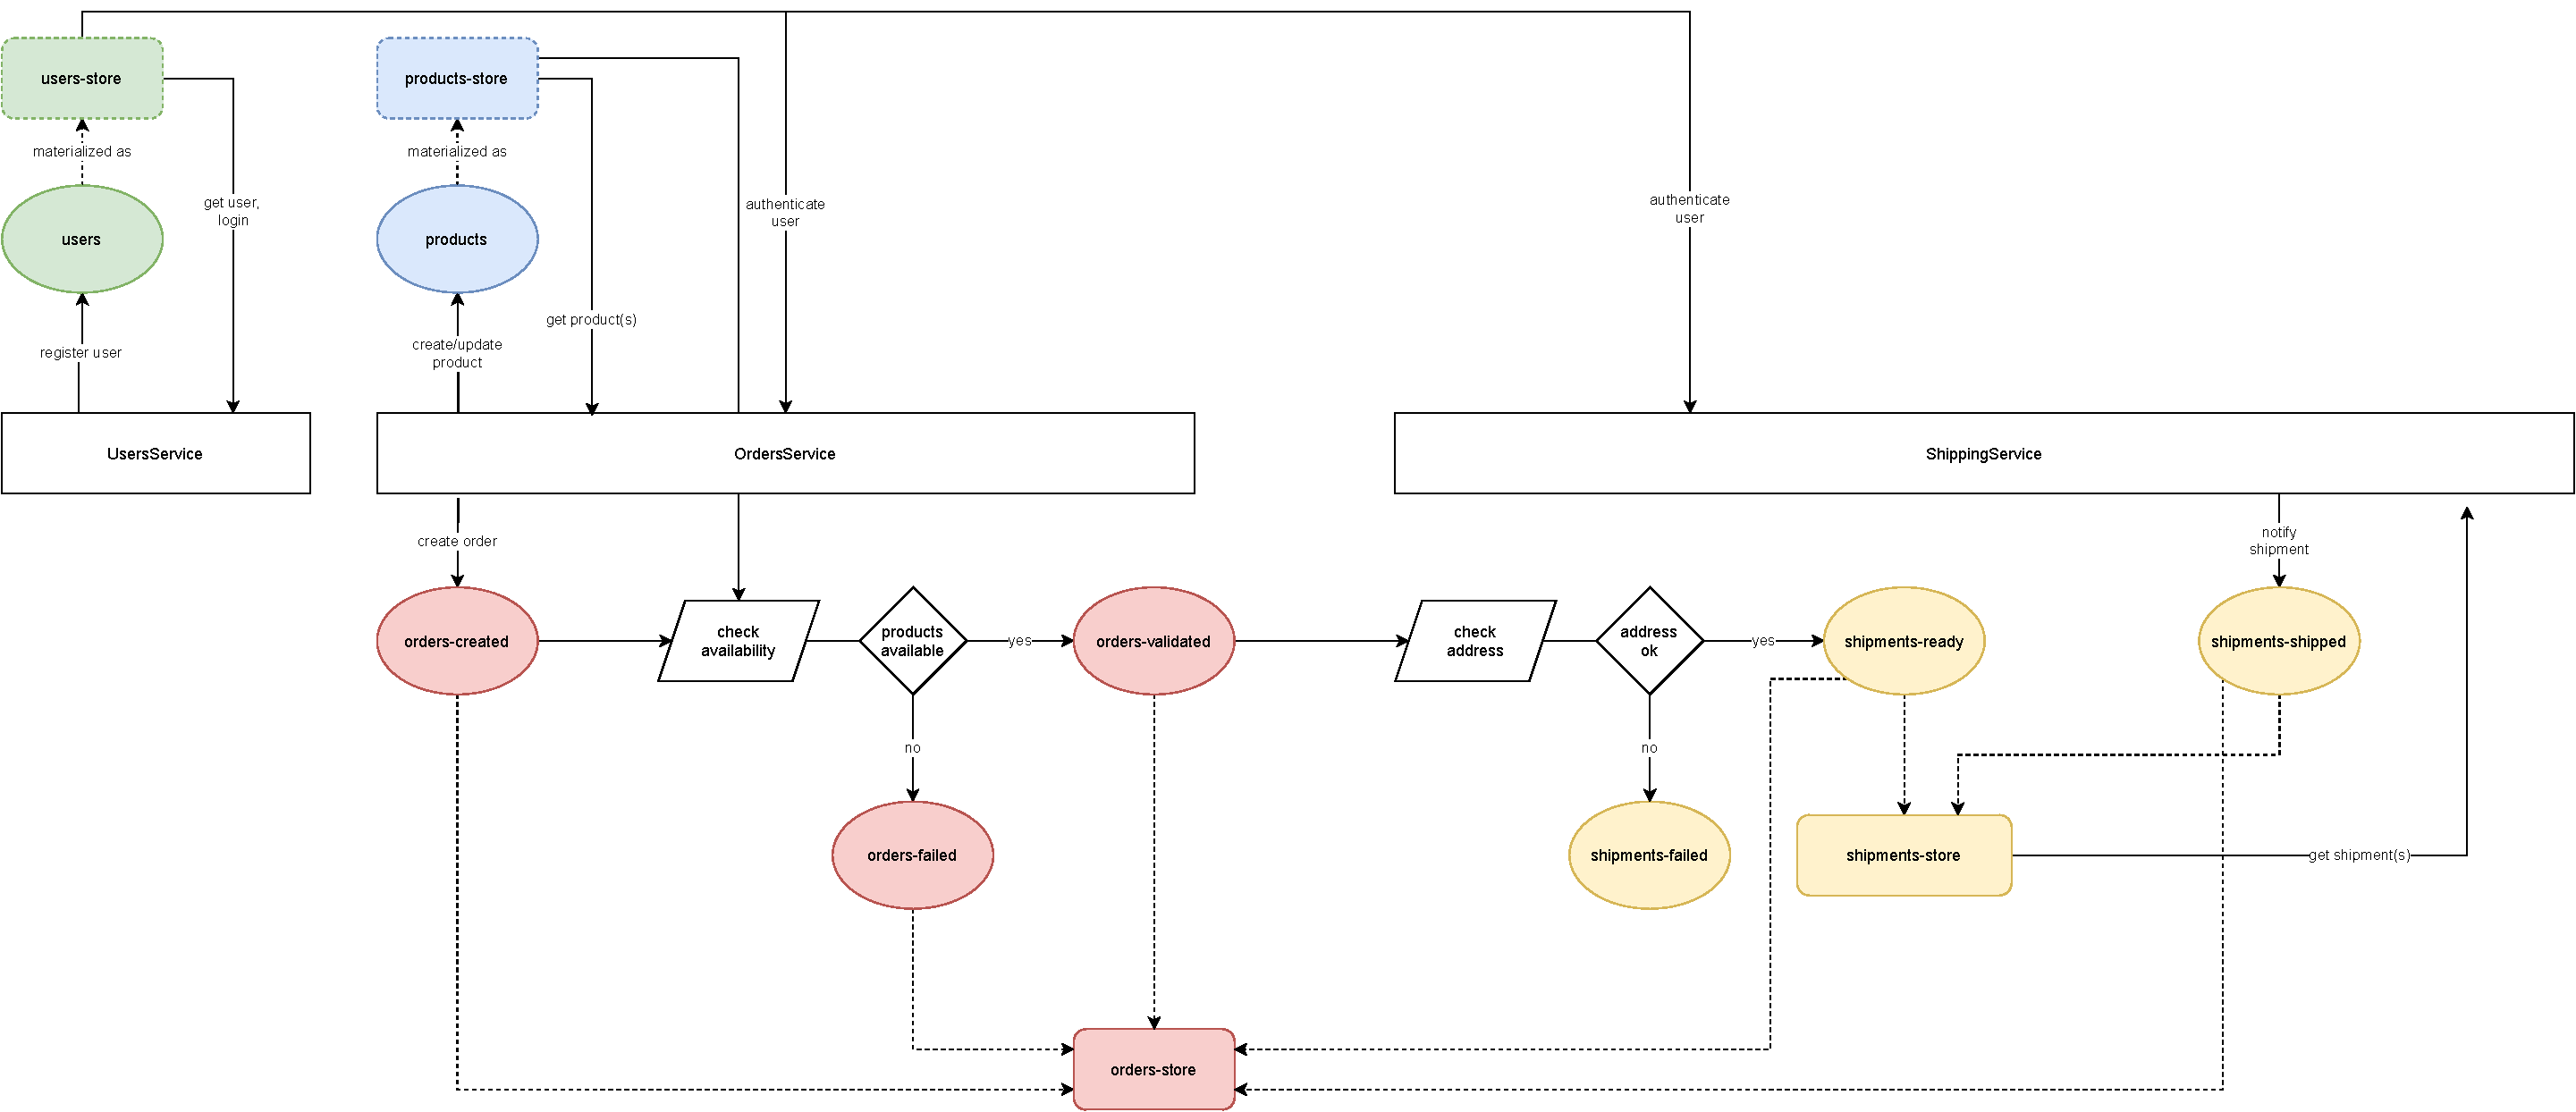
\includegraphics[width=\textwidth]{dataflow_diagram_1}
    \caption{Data flow with different topics for each state of the order (solution 1)}
    \label{fig:dataflow_diagram_1}
\end{figure}

\begin{figure}[p]
    \centering
    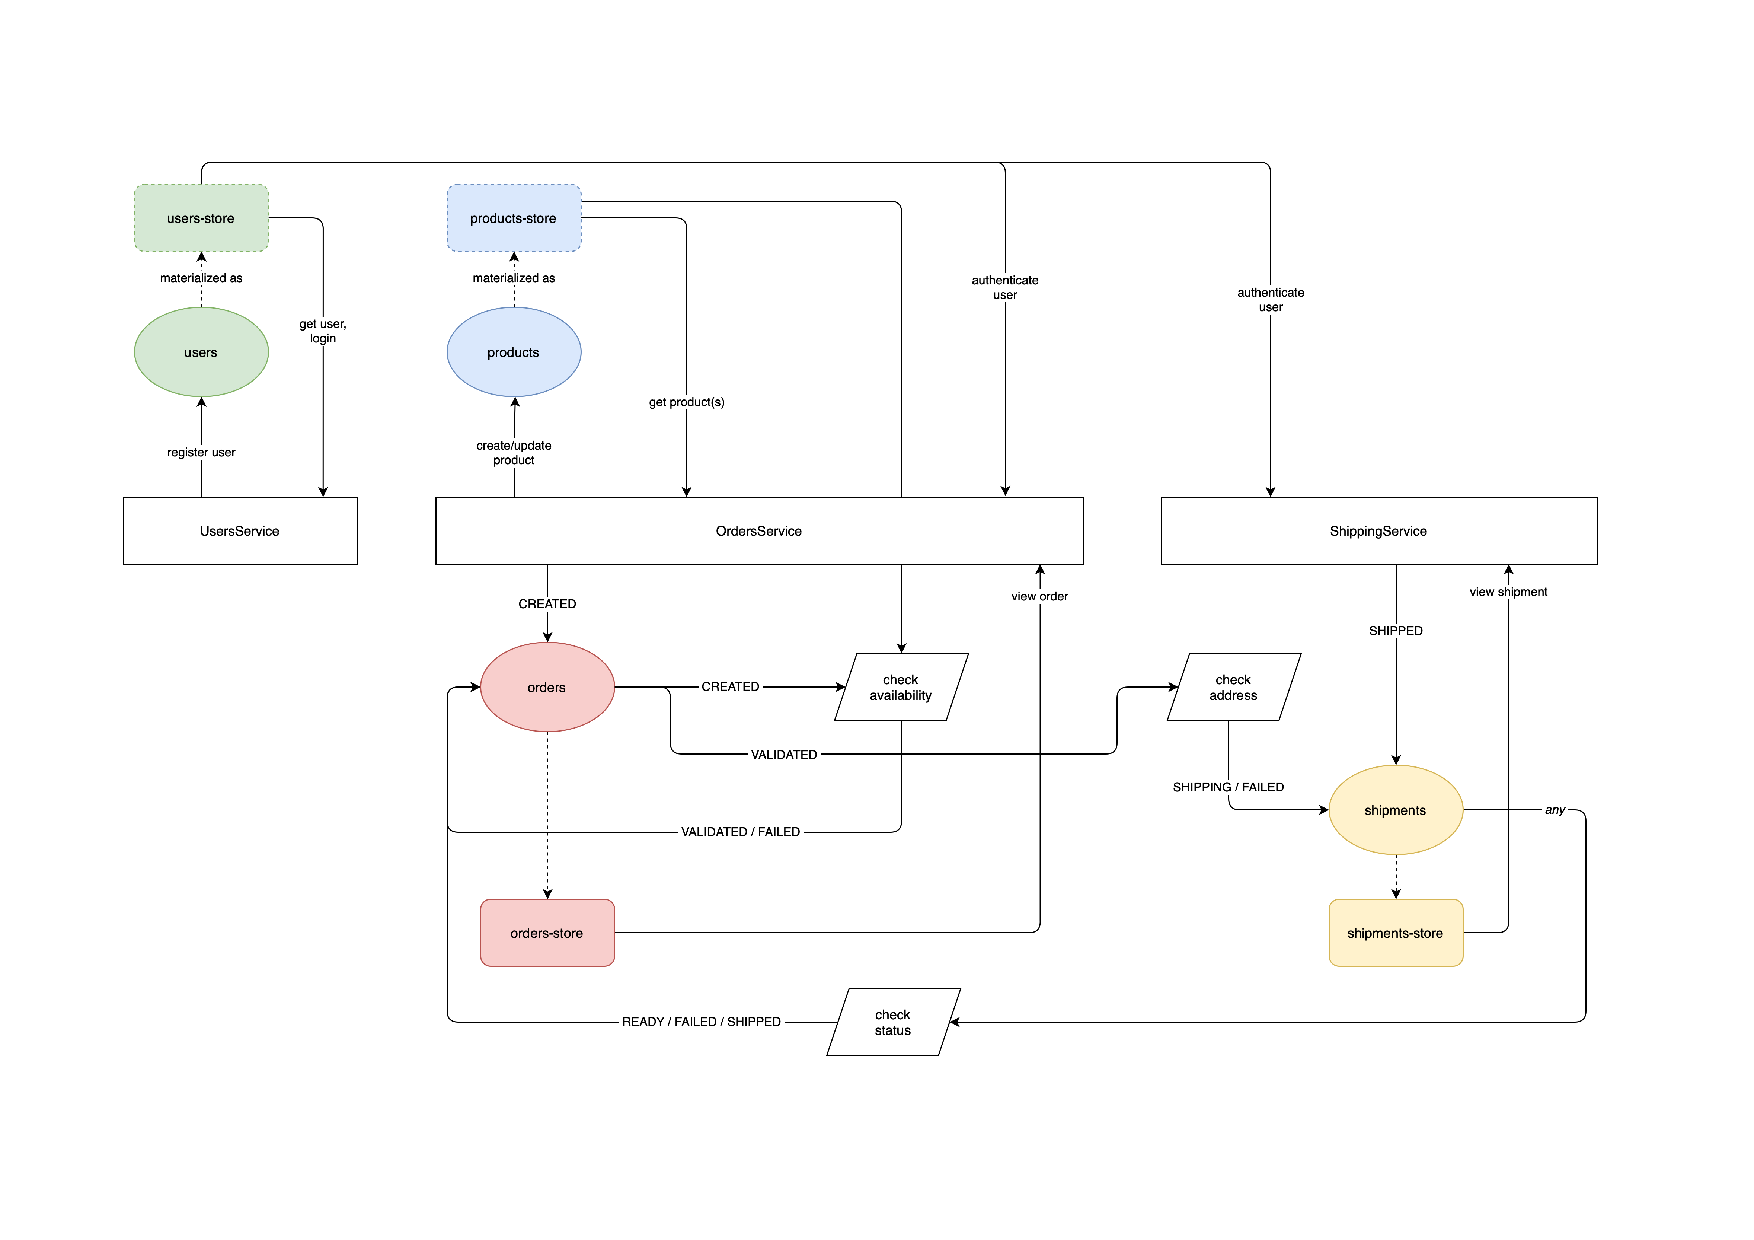
\includegraphics[width=\textwidth]{dataflow_diagram_2}
    \caption{Data flow with only the orders and shipments topics (solution 2)}
    \label{fig:dataflow_diagram_2}
\end{figure}

\subsection{Producers and streams}

In the diagram of figure~\ref{fig:dataflow_diagram_2} we can distinguish two modalities in which a record can be sent to a topic:
\begin{itemize}
    \item The record may be produced as a response to a \emph{user action}, and possibly require the lookup of a previous record (e.g.\ when an admin changes the availability of a product). We implemented this behavior using a transactional producer, committing each record individually. This ensures that, for example, when the user issues a \texttt{POST} request to create an order, if he gets a positive response it means that the order has been successfully stored in the topic. Using transactions at this stage is also the starting point to enable exactly-once semantics.
    \item The record may be produced as part of a \emph{consume-transform-produce} pattern (the parallelograms in the diagram). In this case we would need
    \begin{enumerate*}[label=(\roman*)]
        \item a \emph{consumer} with isolation level set to read-committed,
        \item a transformation that might need to query a state store
        (e.g.\ validating an order requires checking the availability of items),
        \item a \emph{transactional producer} that sends the information to the output topic(s); since it is producing records as a reaction of reading other records, it needs to include the offsets of the consumed records in the transaction.
    \end{enumerate*}
    \break
    Instead of setting up these manually, we chose to use the \emph{Kafka Streams API} that does exactly the things detailed above, but results in fewer and more readable code. Let's take order validation for example:
    \begin{enumerate*}[label=(\roman*)]
        \item we create a stream from the orders' topic,
        \item we filter the records with \texttt{state == CREATED},
        \item we perform the validation with a \emph{stateful transformer} that reads from the products' store and creates a new order record with the appropriate state
        \item we send the new record to the shipments' topic.
    \end{enumerate*}
    We also need to configure the streams to use exactly-once semantics to get the transactional behavior we previously described.
\end{itemize}
\pagebreak

\subsection{Tables and state stores}

As we previously mentioned we often need to query our topics as \emph{tables}, similarly to what we would do in a database. Kafka Streams provides the facilities to read such tables from topics, treating them as update logs.
These tables are \emph{materialized} by state stores, which are built locally on the clients (our microservices).

There are two choices, w.r.t.\ partitioning: a \emph{KTable} is populated from a single partition of a topic, while a \emph{GlobalKTable} is populated from all partitions.
In our application — since each service might be replicated — we always need a global view on things, so we always used \emph{GlobalKTables}.

This choice ensures that all data that might be needed is always locally available in each replica, but at the cost of keeping it in memory/disk. We are aware that this limits the scalability of the system, so we'll take a look at how the design can be improved.

If we choose to use a \emph{KTable} we will create a consumer group for each microservice, so that each replica of that microservice gets a partition. Since we want each replica to be able to answer any query from the outside, we have two possibilities:
\begin{enumerate}
    \item We partition the data such that the data for each query can be found on a single partition. In this case the replica that receives the request will first determine which replica will be able to answer the query (Kafka provides a metadata service to do this) and forward the request to it, acting as a proxy.
    \item The replica that receives the request performs the query locally and forwards them to all the other replicas, then it waits for the responses and aggregates the results.
\end{enumerate}

\noindent
Notice that in our application one might need to query a table for two reasons:
\begin{itemize}
    \item To directly provide a response to the user, i.e. when answering a \texttt{GET} request for users, products, orders or shipments. In these cases we might be able to use some clever partitioning and employ strategy (1).
    \item As part of another operation, which is true for \emph{products} (to check their availability while validating an order) and for \emph{users} (for authentication). In these cases it is much better to avoid partitioning, since it would likely require to use strategy (2) which slows down the process.
\end{itemize}
In this spirit, we think that the tables for \emph{users} and \emph{products} shall not be partitioned in any of the services. By contrast, \emph{orders} and \emph{shipments}, which will likely grow faster, can be efficiently partitioned.

The \emph{orders} can be partitioned by customer. The key is \texttt{customerId:uuid} so, if we partition based on the hash of \texttt{customerId}, when a customer asks for all of his orders, we can then ask Kafka's metadata service for the location of key \texttt{"customerId:"} and be sure that such replica will contain all the orders for that customer.

Currently, there is no distinction between \emph{shipments} and orders. However, if the system is to scale, we expect that a shipment will be assigned to a specific delivery man, therefore we can partition the topic by \texttt{deliveryManId}, similarly to before.

\todo[inline]{Add explanation of how we achieve fault tolerance}
\todo[inline]{Compare and contrast in memory vs. persisted state stores (?)}
\todo[inline]{Add reference for the REST API}